\chapter{State of the Art} \label{chap:sota}

This chapter presents the fundamental concepts of underwater acoustics engineering for localization and positioning of aquatic autonomous vehicles.

\section{Underwater acoustic channel} \label{sec:acoustchann}

Although satellite based navigation systems are the most commonly used for positioning and localization at the air, the used radio signals are highly absorbed by the water and thus inappropriate for underwater localization and also for communications. Therefore, the state of the art solutions for long range localization and communications rely on the propagation of acoustic signals.

The natural limitations of acoustic channels combined with the properties of an underwater environment, result in challenges and limitations in developing communication and localization systems \cite{survey-tech-chall}:
\begin{itemize}
	\item Long propagation delays;
	\item Variable speed of the acoustic signals;
	\item Reference nodes may have different drifting rates from each other due to water currents, which leads to uncertainties on the definition of absolute times and synchronization;
	\item Limited bandwith
	\item Signals are bended due to sound speed variation along the water column and shadowed in many different surfaces, which may lead to the incorrect detection of the line-of-sight (LOS) signal;
	\item Attenuation and asymmetric signal-to-noise ratio, which arises from SNR depending on depth and frequency with complex behaviors that depend on the characteristics of the environment;
\end{itemize}

\subsection{Speed of sound} \label{subsec: speed-sound}

The oceanic environment has a complex sound propagation model, as it comprises many variants in order to realistically represent underwater acoustics.

Acoustic signals' propagation speed is mainly related with two factors: compressibility and density. The water density can be characterized by the temperature, salinity and pressure,which is associated with depth. Figure \ref{fig:spd-sound} exhibits a generic sound speed profile in relation to depth. The water surface is commonly a mixed layer which results in an approximately constant sound speed. After this layer, it suffers a significative decrease, usually reaching the lower tangible speed, which results from the variation of temperature that characterizes the thermocline layer. From that point forward, pressure is the greatest influencer on the speed of sound, so it increases relatively proportionally to depth .

\begin{figure}[!htbp]
	\centering
	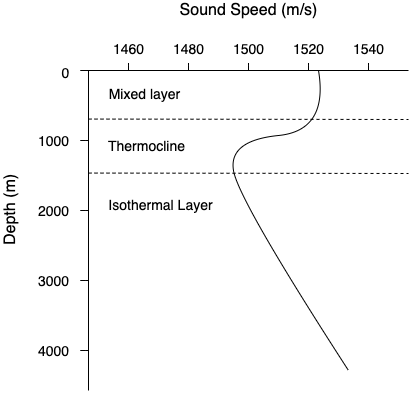
\includegraphics[width=0.6\textwidth]{figures/sound-profile}
	\caption{Generic sound speed profile}
	\label{fig:spd-sound}
\end{figure}

The empirical equation \ref{eq:spd-sound} \cite{ocean-acoust} is a simplified translation of the behavior of the sound speed \textit{c} in meters per second, with relation to the temperature \textit{T} in ºC, the salinity \textit{S} in parts per thousand and the depth \textit{z} in meters. 
\begin{eqnarray}
c = 1449.2 + 4.6T - 0.055T^2 + 0.00029T^3 + (1.34 - 0.01T)(S-35) + 0.016z 
\label{eq:spd-sound}
\end{eqnarray}


\subsection{Multipath} \label{subsec:multipath}

Multipath occurs when a transmitting signal suffers reflection or refraction in a surface (e.g. water surface, ocean floor, dock's wall), leading to a change in its original characteristics. This phenomenon can affect the propagation speed, the energy and the total distance that the signal was predicted to travel. These altered signals in conjunction with constant movement of the receiver makes it more complicated to accurately estimate the distance between the transmitter and the receiver, as well as determine the line-of-sight signal. 

\begin{figure}[!htbp]
	\centering
	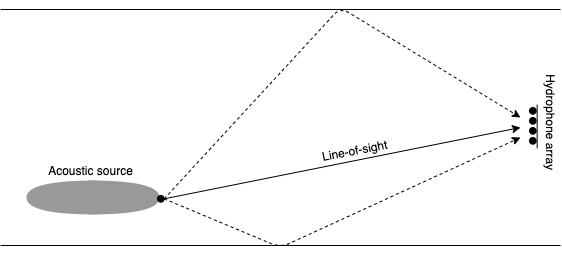
\includegraphics[width=0.7\textwidth]{figures/multipath}
	\caption{Multipath}
	\label{fig:mpath}
\end{figure}

In consequence, the underwater acoustic channel is qualified as a non-minimum phase system because it produces time-variant output responses.

\subsection{Doppler Effect} \label{subsec:doppler}

In a communication and localization system between two entities moving with non-zero relative velocity, if a transmitter sends a signal with a certain operation frequency to the receiver, then the perceived frequency by the receiver will suffer a shift from the original signal. This frequency difference is expressed as a Doppler shift and explained by the Doppler Effect.

The magnitude of the generated frequency shift can be expressed as a ratio \ref{eq:ratio}, where the transmitter-receiver velocity is compared to \(c\), the speed of sound \cite{commchan}.

\begin{eqnarray}
&a = \frac{v}{c}
\label{eq:ratio}
\end{eqnarray}

Autonomous Underwater Vehicles (AUVs) usually move with velocities in the order of few meters per second. Therefore, the \(a\) factor mentioned above has a significant value and needs to be considered when implementing synchronization systems, as well as developing estimation algorithms.

In certain localization and communication systems, it is critical to correct the Doppler effect because data can be compromised (e.g. FSK modulated signals, in which information is codified into frequency changes). A simple Doppler compensation process  was proposed in \cite{thesis-joao}, in a system to detect phase-modulted binary sequences using cross-correlation.

This phenomenon can also be explored to determine the relative velocity between two devices, by measuring the frequency deviation with respect to the frequency expected to be received.


\subsection{Attenuation and signal-to-noise ratio} \label{subsec:snr}

When considering underwater communication systems, it is essential to quantify the attenuation of the channel, i.e. the part of the signal's energy which is absorbed by the involving surrounding. In underwater channels, this absorbance is frequency variable and it is also dependent on physical characteristics of the water, as salinity and temperature. 

The underwater acoustic channel has a particular model that describes its attenuation path loss \(A(d,f)\), given in logarithmic scale by equation \ref{eq:attenuationdb} \cite{pathloss}. 
\begin{eqnarray}
&10\ log(A(d,f)) = 10\ k\ log(d) + d\ 10\ log(a(f))
\label{eq:attenuationdb}
\end{eqnarray}
From the equation, \(d\) is the distance from the transmitter to the receiver in kilometers (Km), \(f\) is the operating frequency in kilohertz (KHz), \(10klog(d)\) represents the spreading loss which describes how the sound level (in decibel, dB) decreases as the sound wave spreads, \(d10log(a(f))\) is the absorption loss that a signal suffers during its propagation path, \(k\) is the spreading factor which is related with the considered configuration (e.g. cylindrical, spheric, etc.), \(a(f)\) is the absorption coefficient that can be obtained through the equation in \cite{pathloss}.

Noise is another factor that is considered when analyzing a real underwater acoustic channel, as it defines the signal-to-noise ratio (SNR) that characterizes the channel. The SNR is dependent on the attenuation level which increases with frequency, and the noise which decays with frequency. Consequently, the SNR varies over the signal bandwidth and it is asymmetric. The equation \ref{eq:snr} \cite{commchan} expresses this relationship, where \(S_{d}(f)\) represents the power spectral density of the transmitted signal.
\begin{eqnarray}
&SNR(d,f) = \frac{S_{d}(f)}{(A(d,f))\ N(f)}
\label{eq:snr}
\end{eqnarray}

%________________________________________________________

\section{Range estimation for underwater localization}

Underwater localization takes into consideration the distance between the target object to track and the reference point. As consequence, it is always relevant to apply methods which easily and effectively determine this range.

There are two main types of techniques that are used to achieve such objective: the Received Signal Strength Indicator (RSSI) and the Time Delay Estimation (TDE).


\subsection{Received Signal Strength Indicator}

The Received Signal Strength Indicator (RSSI) method is based on the strength of the signal that reaches the target. It determines the distance between the target and the reference node by analyzing the received signal strength and comparing it with an underwater attenuation model which is range dependent [\hyperref[r:ocean-acoust]{3}]. 

Since the underwater acoustic channel suffers from multipath, time variance and high overall path loss, the RSSI technique is not adequate for underwater applications.

\subsection{Time Delay Estimation}
Time Delay Estimation (TDE) mechanisms use a pair of nodes, the target and the reference point, to measure the range between them. This distance is based on the time that it takes for a signal to travel from the reference point to the target.

There are three main categories that devide TDE methods, which are Time Difference of Arrival (TDOA), Time of Arrival (TOA) and Time of Flight (TOF).

\subsubsection{Time of Arrival}

Time of Arrival (TOA) is interpreted as the time delay between the transmission of a signal in the reference node until its reception on the target node. Although this is the conceptually simplest method to employ, it requires synchronization between the nodes since the target entity needs to know the instance when the signal was sent to be able to calculate the difference.

Considering a generic transmitted signal \textit{s(t)}, the received signal can be expressed as \ref{eq:toa}, where $\tau$ represents the time of arrival and \textit{n(t)} is white noise with zero mean \cite{wirelesscomm}. 

\begin{eqnarray}
& r(t) = s(t - \tau) + n(t)
\label{eq:toa}
\end{eqnarray}

\subsubsection{Time Difference of Arrival}

The Time Difference of Arrival (TDOA) is a technique that compares the time of arrival of a signal to different hydrophones in order to estimate the angle of arrival of the acoustic signal. The array of reception hydrophones have known determined positions among them so that is is possible to compare the different times of arrival or phase differences. This method can be employed using a uni-directional signal or a round trip communication.

There are several algorithms and mathematical models that can be employed to execute the TDOA method, such as the Cross-Correlation and Maximum Likelihood.

\subsubsection{Generalized Cross-Correlation}

The Generalized Cross-Correlation (GCC) method is used to generically represent the relationship strength between two signals.

Considering two distanced hydrophones in the same environment and an acoustic source \textit{s(t)}, \textit{x1(t)} and \textit{x2(t)} are the signals received by each of the two hydrophones. The equations \ref{eq:gcc1} and \ref{eq:gcc2} \cite{crosscorr} express the mentioned signals in relation to \textit{w1(t)} and \textit{w2(t)} which are Gaussian noise coefficients uncorrelated with the source, $\tau$ that represent the delay and $\alpha$ which is an attenuation function.
\begin{eqnarray}
&x1(t) = s(t) + w1(t)
\label{eq:gcc1}\\
&x2(t) = \alpha s(t - \tau) + w2(t)
\label{eq:gcc2}\\
\end{eqnarray}

From these expressions, the generalized cross-correlation function between signals \textit{x1(t)} and \textit{x2(t)} is given by \ref{eq:gcc3}. The $G_{x1x2}(f)$ is the spectrum of the cross-correlation. The $\psi(f)$ represents a prefilter and it is essentially the distinctive parameter that originate various different methods of cross-correlation, since it should depend on different environments and properties as SNR. 
\begin{eqnarray}
& R_{x1x2}(\tau) = \int_{-\infty}^{\infty} \psi(f) G_{x1x2}(f)\ e^{i2\pi f\tau} df
\label{eq:gcc3}\\
& T = \tau_{max} [ R_{x1x2}(\tau) ]
\label{eq:gcc4}
\end{eqnarray}

Finally, the maximum value of $R_{x1x2}(\tau)$, expressed in \ref{eq:gcc4}, is the so called correlation peak and provides information about the time delay $\tau$ which is the main matter of Time Delay Estimation. 


\subsubsection{Cross-Correlation}

After approaching the generalized method of cross-correlation, it is possible to better understand the Cross-Correlation (CC) method. There are two main variations of CC \cite{crosscorr}, which are the slow cross-correlation in the  time domain and the fast cross-correlation in the frequency domain. The second approach is based on the Fast Fourier Transform as it locates the peak by analyzing frequency similarities between the signals. 

Th Cross-Correlation technique uses a prefilter $\psi(f)$ equal to 1, as it is the simplest method of its kind.

\subsubsection{Maximum Likelihood}

The Maximum Likelihood (ML) method is a variation of Cross-Correlation which uses the prefilter $\psi(f)$ represented mathematically by \ref{eq:ml1}, where $\gamma_{12}(f)$ is a function of spectrum of cross-correlation $G_{x1x2}(f)$ and spectrum of auto-correlations $G_{x1x1}(f)$, $G_{x2x2}(f)$ as expressed in \ref{eq:ml2} \cite{crosscorr}.

\begin{eqnarray}
& \psi(f) = \frac{|\gamma_{12}(f)|^2}{|G_{x1x2}(f)|[1-|\gamma_{12}(f)|^2]}
\label{eq:ml1} \\
& |\gamma_{12}(f)|^2 = \frac{|G_{x1x2}(f)|^2}{G_{x1x11}(f) . G_{x1x11}(f)]}
\label{eq:ml2} 
\end{eqnarray}

There is also a version of ML that uses the power spectral densities of the signals, which can be helpful for calculations in various applications. 

\subsubsection{Time of Flight}

Time of Flight (TOA) measures essentially the round-trip time communication between two nodes. The target node sends a signal to the reference node, which has an integrated transponder that responds transmitting a signal back to the target. T4he TOA is then estimated as the time interval from the moment the first signal is transmitted until the moment the second signal is received by the same node. 

This method may be used without additional synchronization systems as it assumes that the response signal is sent immediately after the received one and the intrinsic transmitting delays are known.

The accuracy of this technique depends mainly on the environment conditions, which include the water properties and the surrounding reflection surfaces which cause multipath. Therefore, the mechanism is susceptible of variable errors according to the location and characteristics of its employment.

%________________________________________________________

\section{Localization estimation}

In networks with multiple nodes is typical to use localization estimation to establish position relationships between elements. The operation principal is usually to have a set of reference nodes with known positions so that it is possible to determine the relative positions between each reference node and the target. 

An extensive comparison of different localization schemes for underwater sensors networks can be consulted in \cite{suvey-loc}.

\subsection{Triangulation}

Triangulation is a method of localization based on the measurement of angles which are related to the reference beacons and the target object. 

\subsubsection{Three-Object Triangulation}
The simplest method of this category is the Three-Object Triangulation, which considers a configuration as illustrated in figure \ref{fig:tri1}. It is assumed that the location of the beacons is pre-configured and the environment is obstacle-free. $\lambda_{12}$ is the angle formed by the intersection of the straight lines [O,1] and [O,2]. Similarly, $\lambda_{31}$ is the angle formed by the intersection of the straight lines [O,1] and [O,3]. Using these two sets of nodes, we can trace circumferences that include their coordinates and as a consequence their intersection will correspond to the location of the target.

\begin{figure}[!htbp]
	\centering
	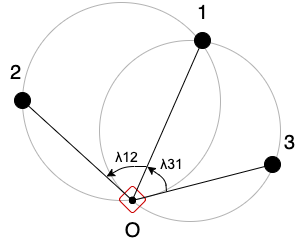
\includegraphics[width=0.4\textwidth]{figures/triangulation}
	\caption{Three-Object Triangulation}
	\label{fig:tri1}
\end{figure}

Although this is a very straightforward technique to implement, it does not cover all possible scenarios, namely when the three beacons and the object are all placed in the same circumference or when the environment has obstacles between nodes.

\subsubsection{Geometric Triangulation algorithm}

A more complex method relies on the Geometric Triangulation algorithm. 

\begin{figure}[!htbp]
	\centering
	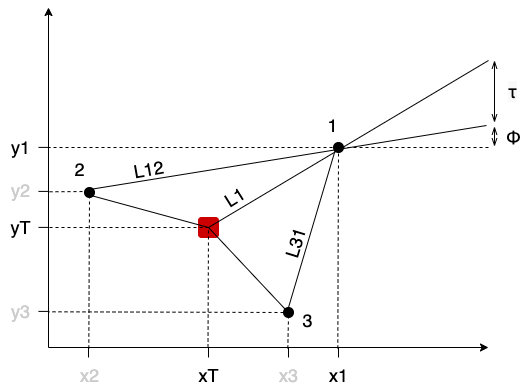
\includegraphics[width=0.5\textwidth]{figures/geotriang}
	\caption{Geometric Triangulation algorithm}
	\label{fig:tri2}
\end{figure}


Considering a Cartesian plane with defined lengths L1, L12 and L31, as shown in image \ref{fig:tri2}, it is possible to establish trigonometrical relationships that estimate the location of the object within the created triangular areas. The position of the target is given by coordinates (xT,yT) and can be calculated through equations \ref{eq:tri1} and \ref{eq:tri2}. (x1,y1) represents the location of beacon 1 and L1 is the distance between this beacon and the object. The trigonometric relationships for calculating the mentioned variables can be consulted in \cite{triangalgo}.

\begin{eqnarray}
& xT = x1 - L1 * cos(\phi + \tau)
\label{eq:tri1}\\
& yT = y1 - L1 * sin(\phi + \tau)
\label{eq:tri2}
\end{eqnarray}

\subsection{Trilateration}

Trilateration is a technique that does not rely on calculations using angles but instead it uses distances to locate an object.

Considering a scenario with three reference beacons, the distance between the target and each one of the beacons is taken as the radius of a circumference. By doing this, it is possible to obtain three circumferences that intersect each other. With only two circumferences, there are two possible locations for the object, however, when added the third circumference the exact location is obtained. The 2D coordinates are obtained by solving systems of equations with the circle equation \ref{eq:circle} \cite{trilat}, where $(x_{i}, y_{i})$ is the beacon coordinates and $r_{i}$ is the distance between the beacon and the object.

\begin{eqnarray}
& (x - x_{i})^2 + (y - y_{i})^2 = r_{i}^2 
\label{eq:circle}
\end{eqnarray}

Trilateration is commonly used in underwater acoustic localization, as it used to find a relative position of the target in two dimensions and additionally determines the depth as third dimension, by using a pressure sensor with high accuracy.

\subsection{Multilateration}

Multilateration is a generalization of the trilateration technique, as it uses the same conceptual principal with multiple reference beacons instead of exactly three. In this method, the employment of \textit{n+1} nodes will allow to determine \textit{n} coordinates \cite{arch_localiz}. For example, determining the position (x,y,z) of a target, would require to resolve a system of equations using \ref{eq:mult}. $(x_{i}, y_{i}, z_{i})$ is the coordinates of the beacon and $d_{i}$ is the distance between the beacon and the target.

\begin{eqnarray}
& (x - x_{i})^2 + (y - y_{i})^2 + (z - z_{i})^2 = d_{i}^2 
\label{eq:mult}
\end{eqnarray}

Distributed mechanisms, such as multilateration, are usually divided in three phases of positioning \cite{suvey-loc}:
\begin{itemize}
	\item Distance estimation between the reference nodes and target object, usually using TDOA or TOF mechanisms;
	\item Position estimation, usually obtained by solving a system of linear equations through mathematical efficient techniques;
	\item Final refinement of the measurement in order to improve accuracy.
\end{itemize}

As an alternative to solve localization issues using circumferences, multilateration can also take advantage of a hyperbola-based localization method. Considering a target at (x,y) and three reference beacon with coordinates $(x_{i},y_{i})$,  $(x_{j},y_{j})$ and  $(x_{k},y_{k})$, we have that the difference between times of arrival $t_{i}$ and $t_{j}$ to nodes $i$ and $j$, respectively, can be related to the distance between nodes, as expressed in \ref{eq:hyper} \cite{arch_localiz}. $d_{i}$ and $d_{j}$ are the distance from node $i$ and $j$, respectively, to the target object. 

\begin{eqnarray}
& d_{i} - d_{j} = c * (t_{i} - t_{j}) = \sqrt{(x - x{i})^2 + y - y{i})^2} - \sqrt{(x - x{k})^2 + y - y{k})^2}
\label{eq:hyper}
\end{eqnarray}

%________________________________________________________

\section{Positioning Systems}

Positioning systems are used to track the underwater position of a vehicle or other object, in relation to reference structures of transponders called \textit{baseline stations}. These systems are classified based on the distance between the baseline stations. The configurations that will be explained are Long Baseline (LBL), Short Baseline (SBL), Ultra Short Baseline (USBL) and the inverted versions of all above.

\begin{figure}[!htbp]
	\centering
	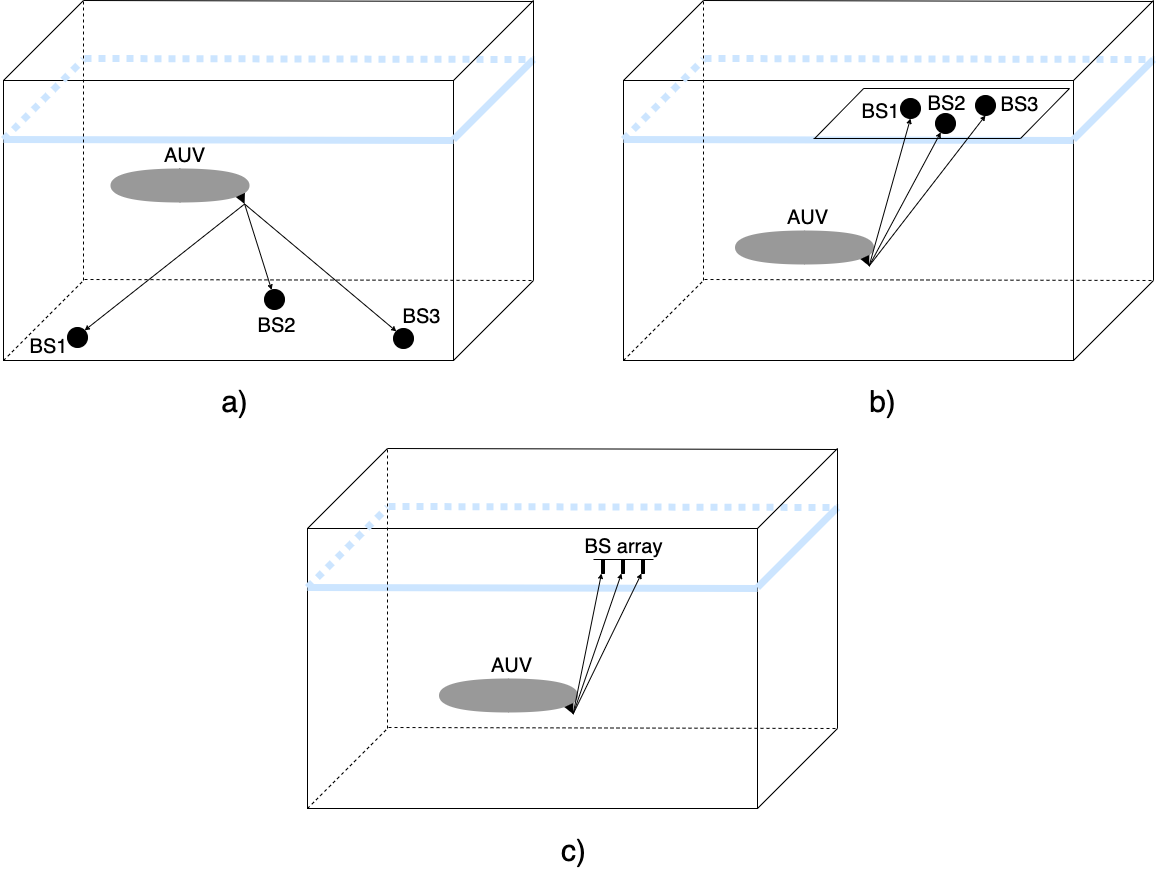
\includegraphics[width=1\textwidth]{figures/lblsblusbl}
	\caption{Generic configuration of: a) LBL; b) SBL; c) USBL}
	\label{fig:lblsblusbl}
\end{figure}

\subsection{Long Baseline (LBL)}

Long Baseline systems use a positioning method with large distances between baseline stations, with range typically from 50m to more than 2000m  and usually similar to the distance between object and transponders [\hyperref[r:survey-tech-chall]{3}]. A typical LBL configuration is represented in figure a) \ref{fig:lblsblusbl}.

The LBL method uses at least three transponder stations deployed usually on the sea floor, allowing to execute trilateration. Additionally, a transducer is integrated on the object to be tracked. 

A complete localization procedure starts with the vehicle sending an acoustic signal which is received by the transponders. Thereafter the transponders transmit a response and, by analyzing the Time of Flight of the communication, the system can determine the distance between the vehicle and each base station. Then the relative position of the vehicle is determined through trilateration. Additionally, if the transponders have known geographic positions, it is possible to infer the vehicle geographic position. 

As this technique presents large distances between the object and the base stations, the typical 1m to few centimeters accuracy is considered to be high because it will not compromise the localization of the vehicle. 


\subsection{Short Baseline (SBL)}

Short Baseline systems are characterized by having distances around 20m to 50m between baseline stations \cite{survey-tech-chall} and use an operation procedure similar to the LBL method. However, the transponders are usually placed in a moving platform, which assures a fixed relative position between them. A typical SBL configuration is represented in figure b) \ref{fig:lblsblusbl}.

The position of the vehicle to be tracked can be determined by translating the Time of Flight between the multiple transponders and the object into a distance value, which is achieved by equation \ref{eq:sbl} \cite{sbl}. The $t_{i}$ corresponds to the propagation time of the signal from the vehicle to the \textit{i}th transponder, \textit{c} is the speed of sound, [$x_{b_{i}}$, $y_{b_{i}}$ and $z_{b_{i}}$] is the coordinate position of the transponder.

\begin{eqnarray}
&\sqrt{ (x_{b_{i}}-x)^2 + (y_{b_{i}}-y)^2 + (z_{b_{i}}-z)^2 } = c\ *\ t_{i}
\label{eq:sbl}
\end{eqnarray}

In a SBL system, when the distance between baseline stations is increased the accuracy improves and, contrarily, when the mentioned distance decreases the accuracy deteriorates, which can raise some deployment challenges.

\subsection{Ultra Short Baseline (USBL)}

Ultra short baseline systems are composed essentially by one baseline station, with an array consisting of several traducers distanced typically less than the wavelength \cite{lblsblusbl}, and a transponder integrated on the object to be tracked. It is usually used in underwater positioning in shallow areas of the sea, as represented in figure c) \ref{fig:lblsblusbl}.

Similarly to the previously mentioned procedures, the USBL positioning method relies on the Time of Flight of the exchanged signals. However, the traducers are too spatially close from each other to execute an accurate trilateration. Instead, it is measured the phase difference or time-delay difference of the received signal between every traducer, in order to estimate the azimuth and distance to the acoustic source. 

Assuming a three dimensional scenario for the positioning system, as represented in figure \ref{fig:usblgeo}, the object's coordinates are given by equations \ref{eq:usblgeo1}, \ref{eq:usblgeo2} and \ref{eq:usblgeo3} \cite{usbl-new}. The $\lambda$ corresponds to the wavelength of the of the transmitted signal which depends on its operation frequency, \textit{f}, and it is affected by the speed of sound \textit{c}, as represented equation \ref{eq:cfw}.
The \textit{d} represents the distance between hydrophones, $\psi_{12}$ and $\psi_{22}$ are the phase difference between H2 and the other two hydrophones, \textit{H} is the height of the target object, \textit{X} is the distance of the target along the x-axis direction, \textit{Y} is the distance of the target along the y-axis direction and \textit{l} is the slant distance of the target to the hydrophone.
\begin{eqnarray}
& c = f * \lambda
\label{eq:cfw}
\end{eqnarray}
\begin{eqnarray}
& l^2 = X^2 + Y^2 + H^2 
\label{eq:usblgeo1}\\
& \psi_{12} = \frac{2\pi}{\lambda}[\sqrt{l^2} - \sqrt{(d-X)^2 + d^2 + H^2}]
\label{eq:usblgeo2}\\
& \psi_{22} = \frac{2\pi}{\lambda}[\sqrt{l^2} - \sqrt{X^2 + (d-Y)^2 + H^2}]
\label{eq:usblgeo3}
\end{eqnarray}

\begin{figure}[!htbp]
	\centering
	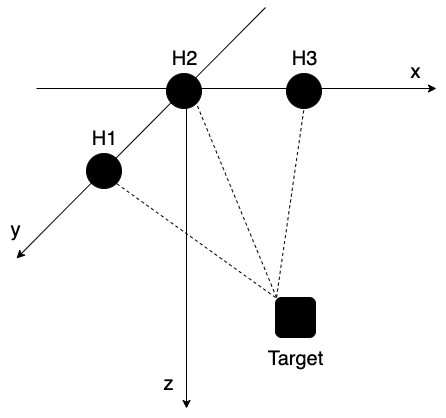
\includegraphics[width=0.5\textwidth]{figures/usbl-config}
	\caption{USBL system configuration}
	\label{fig:usblgeo}
\end{figure}

This is a broadly used technique due to its convenient set up, which allows to have predefined measurements in the order of tens of centimeters and does not require AUV navigation area for the deployment. However it presents the lowest accuracy, comparatively with LBL and SBL, since an error of few centimeters can be realistically corresponding to an inaccuracy of several meters in the position of the object to be tracked.

\subsection{Inverted Systems}

All the previously mentioned positioning techniques use a configuration in which the vehicle to be tracked has a single transducer and there is an external set of transponder to determine the positioning of the said object. However, there is the possibility to benefit from the inverse configuration in some applications. Therefore, there are also the iLBL, iSBL and iUSBL methods, which have the same operation principals as LBL, SBL and USBL, respectively.

%________________________________________________________

\section{Commercial Solutions}

There are several commercial solutions for underwater positioning using the ultra-short baseline method. In this section, it will be presented some of the available devices in the market, indicating their main properties and capabilities. Table \ref{tab:solutions} summarizes the systems with most relevance to the present work. The Medium Frequency (MF) bandwidth is attributed to devices whose manufacturer did not specified the actual frequency range.

\textit{Evologics} produces the S2C R USBL series of acoustic modems \cite{evologics1}, with Sweep Spread Carrier (S2C) technology \cite{evologics2} which uses a broad frequency range to propagate over large distances with reduced noise. The devices have a fixed 0.01m slant range accuracy and a 0.1 degree bearing resolution. These are essentially divided into two groups:
\begin{itemize}
	\item High speed mid-range devices: contains the 18/34 transceivers family \cite{evologics3}, which presents various options for the USBL antenna beam pattern and it is optimal for transmission in horizontal channels.
	\item Depth rated long-range devices: includes the 12/24 transceiver \cite{evologics4}, which have a directional (70 degrees) USBL antenna  and it is optimal for transmission in vertical channels.
\end{itemize}

\textit{Sonardyne} markets the Ranger 2 systems. The Micro-Ranger 2 \cite{sonardyne1} is very easy to use without previous experience and it is appropriate for shallow waters, achieving accuracy of 0.2\%. The Mini-Ranger 2 is ideal for nearshore missions and it is  used for simultaneous tracking of various mobile targets, whose position is updated every 3 seconds.

\textit{Applied Acoustics} offers the Easytrak USBL Systems, which includes the processing software for estimating the position. The Alpha Portable 2655 consists in a very compact structure that includes an array transducer and is capable of reaching a 10cm slant range resolution and a 2 degree RMS.

\textit{Kongsberg} produces the HiPAP family of transducers \cite{hipap_hardw}, which can use the Cymbal acoustic protocol (PSK) or the frequency shift (FSK) modulation technique. Particularly the HiPAP 352 is the model with higher number of active transducers and is able to reaches 0.02m of range accuracy.

\begin{table}[t]
	\centering
	\begin{tabular}{|c|c|c c c|}
		\hline
		Company
		& System
		& Bandwidth(kHz)
		& Connection(kbps)
		& Range(m) \\ \hline 
		\multirow{2}{4em}{Evologics} 
		& S2C R 18/34D USBL & 18-34 & up to 13.9 & 3500\\
		& S2C R 12/24 USBL & 12-24 & up to 9.2 & 6000\\
		\hline 
		\multirow{2}{4em}{Sonardyne} 
		& Micro-Ranger 2 & MF & 0.2-9 & 995\\
		& Mini-Ranger 2 & MF & 0.2-9 & 995\\ 
		\hline 
		\multirow{2}{4em}{Applied Acoustics} 
		& Easytrak Alpha Portable 2655 & MF & n.d. & 500 \\
		&  &  &  & \\
		\hline 
		\multirow{1}{4em}{Kongsberg} 
		& HiPAP 352 & 21-31 & n.d. & 5000 \\
		\hline 
	\end{tabular}
	\caption{Overview of commercial solutions}
	\label{tab:solutions}
\end{table}


%_________________________________________________________


%\begin{eqnarray}
%&10\ log(a(f)) = 0.11(\frac{f^2}{1+f^2})+44(\frac{f^2}{4100+f^2})+2.75*10^{-4}f^2+0.003 
%\label{eq:abs_af}
%\end{eqnarray}


%\begin{eqnarray}
%CIF_1: \hspace*{5mm}F_0^j(a) &=& \frac{1}{2\pi \iota} \oint_{\gamma} \frac{F_0^j(z)}{z - a} dz\\
%CIF_2: \hspace*{5mm}F_1^j(a) &=& \frac{1}{2\pi \iota} \oint_{\gamma} \frac{F_0^j(x)}{x - a} dx 
%\label{eq:cif}
%\end{eqnarray}

